\chapter{Einführung Fallstudie iCompany}
\section{Sie kennen die Inhalte der Fallstudie iCompany}
iCompany ist ein virtuelles Handelsunternehmen, welches in der Musikbranche tätig ist. Das Unternehmen hat kürzlich ein Pianohaus übernommen. Es hat 4 Filialen, 5 Kompetenzzentren und 2 Service Ateliers. Diese werden von einem Zentrallager beliefert. Der Hauptsitz liegt in Rotkreuz.
Es werden Musikinstrumente gewartet, ein- und verkauft, repariert und gestimmt.
\begin{figure}
\centering
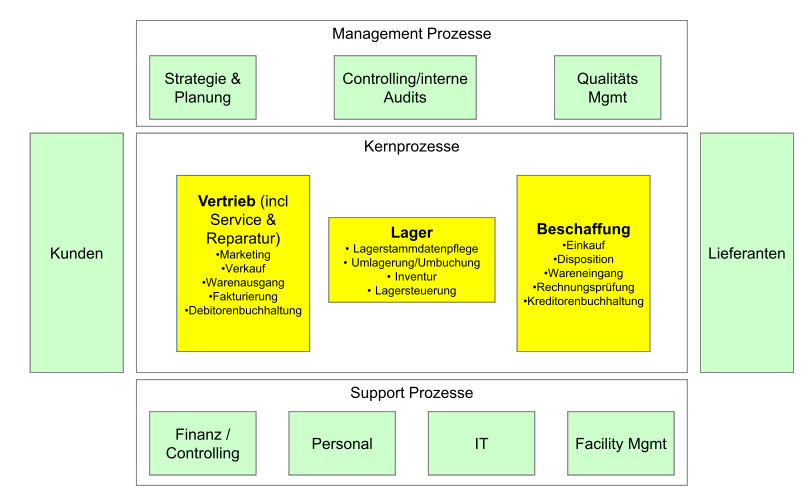
\includegraphics[width=0.9\linewidth]{fig/prozesslandschaft_icompany}
\caption{Prozesslandschaft iCompany}
\label{fig:prozesslandschafticompany}
\end{figure}

Die Departements der Unternehmung sind in Abbildung \ref{fig:organigramm_icompany} ersichtlich.
\begin{figure}
	\centering
	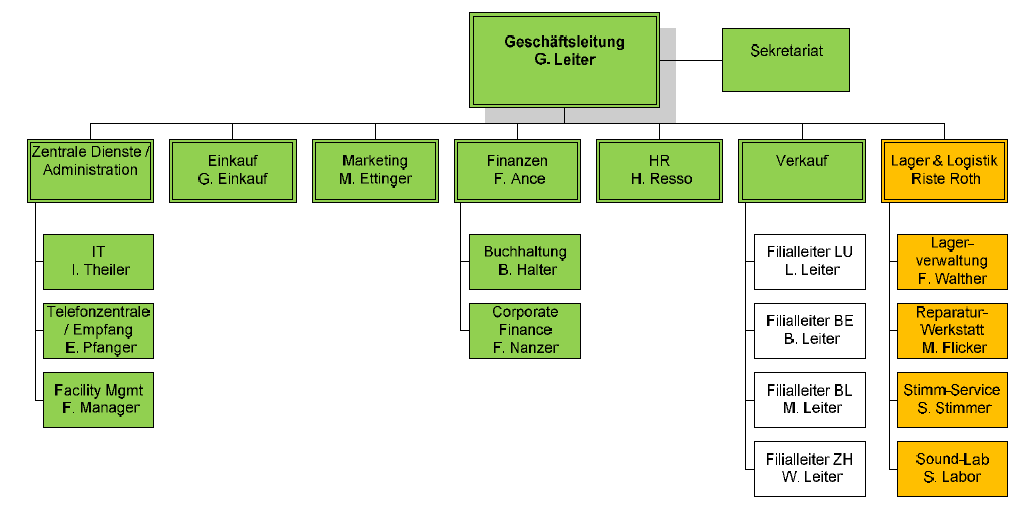
\includegraphics[width=0.9\linewidth]{fig/organigramm_icompany}
	\caption{Organigramm iCompany}
	\label{fig:organigramm_icompany}
\end{figure}

Wichtige Aspekte/Besonderheiten der Unternehmung sind:
\begin{enumerate}
	\item Handel
	\item Mehrere Standorte
	\item Lieferanten im Ausland
	\item Lager
	\item Webshop, Filialen, Telefonsupport
	\item Vor Ort Service
	\item 300 Mitarbeiter
\end{enumerate}

Für die IT werden sich folgende Herausforderungen ergeben:
\begin{enumerate}
	\item Betrieb Webshop (Performance, Ausbau, + ERP System)
	\item Filalnetz (Netzwerktechnische Herausforderung) (gemeinsamer Datenzugriff)
\end{enumerate}
\section{Sie können die grundlegenden Prozesse eines Unternehmens erläutern und in die drei Hauptkategorien einteilen}
Wir haben das Prozessmodell einer Unternehmung, bestehend aus:
\begin{enumerate}
	\item \textbf{Managementprozesse}
		\subitem Strategieplanungsprozess
		\subitem Qualitätsmanagementprozess
		\subitem Controllingprozess
		\subitem Innovationsprozesse
	\item \textbf{Kernprozesse} \\
		Hier findet die Wertschöpfung der Unternehmung statt. Sind von Firma zu Firma unterschiedlich.
		\subitem Innovationsprozess
		\subitem Vertriebsprozess (Leistungsverwertung)
		\subitem Auftragsabwicklungsprozess (Leistungserstellung)
		\subitem Serviceprozess
	\item \textbf{Unterstützungsprozesse}
		\subitem Personalmanagementprozess
		\subitem Finanzmanagementprozess
		\subitem Ressourcenmanagementprozess
		\subitem IT-Managementprozess (IT generell)
\end{enumerate}

\section{Sie kennen den Zweck der IT im Unternehmen und kennen deren Hauptaufgaben}
Die IT ist immer nur Mittel zum Zweck. Die meisten Unternehmen sind keine
Technologie-Unternehmen, die die IT als Kernprozess auflisten.
Sie gilt in den Unternehmen als Unterstützungsprozess und soll demnach auch
die Kernaufgaben unterstützen und optimieren. Mit IT senkt man die Kosten
oder erhöht den Umsatz.